\documentclass[11pt]{article}
\usepackage{xeCJK}
\usepackage[colorlinks,linkcolor=green, anchorcolor=green, citecolor=green]{hyperref}
\usepackage{graphicx}
\usepackage{subcaption}
\usepackage{amsmath}


%opening
\title{深度解读条件随机场\footnote{在自然语言处理领域,由于文本具有序列性,实际只讨论条件随机场(Conditional Random Field, CRF)的一个特例,即线性链条件随机场(Linear Chain CRF)。}}
\author{Yang Fu}

\begin{document}

\maketitle

\begin{abstract}
CRF是概率图模型中极具代表性的概率无向图模型,常用于命名实体识别等序列标注任务。
CRF模型的表达式是对数线性函数,参数包括特征函数及其权重。
训练时,基于前向-后向算法计算正则化后的概率值,然后基于极大似然估计训练模型参数;
推理时,基于维特比算法计算给定观测序列下条件概率最大的标签序列;
实践时,传统机器学习实现版本支持人工显式地定义特征模板,深度学习实现版本在所有位置上共享特征函数并自动学习参数。
相比Softmax,CRF彻底解决标签不一致的问题,缺点是归一化因子计算量较大,同时不能很好处理嵌套和不连续实体。

\end{abstract}

\section{模型推导}

概率无向图模型又称为马尔可夫随机场,它要求$P(Y)$必须满足成对、局部、全局马尔可夫性,然后根据Hammersley-Clifford定理,概率无向图模型的联合概率分布$P(Y)$可以分解成规范化的最大团的势函数乘积\footnote{这里暂不深究Hammersley-Clifford定理,只需明确概率无向图模型的联合概率是由图中最大团的势函数相乘得到的。关于最大团的定义可以查阅图论。}。

序列标注任务的问题定义是:给定给一个序列$x$,计算标签序列$y$的概率$P(y|x)$. 为此,在马尔可夫随机场的基础上引入随机变量X,同时不妨假设Y具有链式结构,便得到线性链条件随机场,此时$P(Y_v|X, Y_w, w \neq v) = P(Y_v|X, Y_v, w \sim v)$,其中$\sim$表示相邻。即Y仍为马尔可夫随机场。

此时:

\begin{equation}\label{key}
	P(Y_i|X, Y_1, ..., Y_{i-1}, Y_{i+1}, ..., Y_n) = P(Y_i|X, Y_{i-1}, Y_{i+1})
\end{equation}

Fig 1展示了两种形式的线性链条件随机场。由于线性链条件随机场的最大团就是相邻两个结点的集合。而通过对这两张图进行内部比较,可以发现左边的图更为特殊,因为X和Y具有相同的结构。现实中,比如对于NER问题,对一个文本序列进行序列标注,都一般假设X和Y具有相同结构,满足左边的那张图。

\begin{figure}[h]
\begin{subfigure}{0.5\textwidth}
	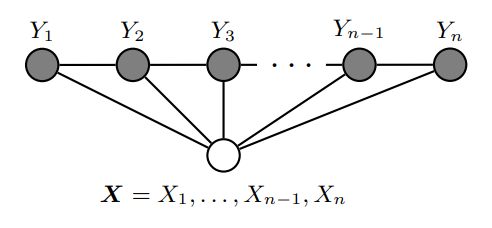
\includegraphics[width=0.9\linewidth]{../images/crf} 
	\caption{仅Y具有链式结构}
	\label{fig:subim1}
\end{subfigure}
\begin{subfigure}{0.5\textwidth}
	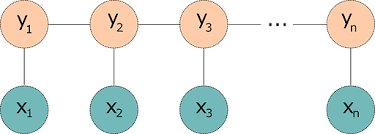
\includegraphics[width=0.9\linewidth]{../images/crf_2}
	\caption{X和Y都具有链式结构}
	\label{fig:subim2}
\end{subfigure}

\caption{CRF架构图}
\label{fig:image2}
\end{figure}

此时,定义CRF中的状态转移特征函数\footnote{特征函数的取值为0或者1.}$t_k(y_{i-1}, y_i, x, i)$和状态特征函数$s_l(y_i, x, i)$作为最大团的势函数,它们分别描述了状态转移概率和发射概率。列举一个具体的特征函数如下:

\begin{equation}\label{key}
	t1(y_{i-1}=1, y_i=2, x, i) = 1, \quad i=2, 3
\end{equation}

这个特征函数其实是可以拆开的,虽然只阐述了在2和3这两个位置上取值为1的条件,但是可以默认其余位置上都为0。

但是光有特征函数是不够的,每个特征函数还都对应一个权重。于是,整个参数化的线性链条件随机场就可以表示为:

\begin{equation}\label{key}
	P(y|x) = \frac{1}{Z(x)}exp(\sum_{i,k}\lambda_k t_k(y_{i-1}, y_i, x, i) + \sum_{i, l}\mu_l s_l(y_i, x, i))
\end{equation}

$Z(x)$是归一化因子,它作用在全局上,实现全局归一化,这恰恰就是CRF相比于MEMM的改进之处。

这里有一个细节值得注意:$i$和$k/l$分别是位置编号和特征函数编号,它们是分开的!换句话说,每个位置上都存在多种特征函数,而一个特征函数又是作用在整个序列$y$上的。

基于此,对CRF进行简化表示:

\begin{equation}\label{key}
	P(y|x) = \frac{1}{Z(x)}exp(\sum_{k=1}^K w_kf_k(y, x))
\end{equation}

其中$f_k(y, x) = \sum_{i=1}^n f_k(y_{i-1}, y_i, x, i)$是两种特征函数的统一形式。

可以看到,$f_k(y, x)$是单个特征函数在整个序列上的取值,$P(y|x)$是所有特征函数与权重的加权和。

这里的特征函数有K个,是两种特征函数的数量和,位置则是从1到n。

接下来,尝试将其转化成向量形式:

\begin{gather*}\label{key}
	P_w(y|x) = \frac{exp(w \cdot F(y, x))}{Z_w(x)} \\
	w = (w_1, w_2, ..., w_K)^T \\
	F(y, x) = (f_1(y, x), f_2(y, x), ..., f_K(y, x))^T
\end{gather*}

这里的$\cdot$表示内积。

简化到这一步还没完,我们还可以将其继续简化到矩阵表示形式。

假设标签的数量为m,定义一个$m$阶矩阵随机变量:

\begin{equation}\label{key}
	M_i(x) = [M_i(y_{i-1}, y_i, x)]
\end{equation}

$M_i(x)$对应在位置$i$处的矩阵,矩阵元素为$M_i(y_{i-1}, y_i, x)$,可展开如下:


\begin{align*}		
	M_i(x) &= [M_i(y_{i-1}, y_i, x)] \\
		&= \begin{bmatrix}
		M_i(y_{i-1}=c_1, y_i=c_1|x) & M_i(y_{i-1}=c_1, y_i=c_2|x) & \cdots & M_i(y_{i-1}=c_1, y_i=c_m|x)\\
		M_i(y_{i-1}=c_2, y_i=c_1|x) & M_i(y_{i-1}=c_2, y_i=c_2|x) & \cdots & M_i(y_{i-1}=c_2, y_i=c_m|x)\\
		\vdots & \vdots & \ddots & \vdots\\
		M_i(y_{i-1}=c_m, y_i=c_1|x) & M_i(y_{i-1}=c_m, y_i=c_2|x) & \cdots & M_i(y_{i-1}=c_m, y_i=c_m|x)
	\end{bmatrix}
\end{align*}

也就是在位置$i$处定义了一个$m*m$的矩阵。

其中

\begin{gather*}\label{key}
	M_i(y_{i-1}, y_i, x) = exp(W_i(y_{i-1}, y_i|x))\\
	W_i(y_{i-1}, y_i|x) = \sum_{k=1}^K w_kf_k(y_{i-1}, y_i, x, i)
\end{gather*}

可以看到$M_i(y_{i-1}, y_i, x)$是一个位置上所有的特征函数的取值的加权和。这里给每个概率加上了一个$exp$,是为了方便计算,加上$exp$之后路径上每个概率连乘,不仅在指数上可以得到累加和,还方便计算softmax概率,后面还会提到。

有了这个$M_i(x)$基本得到了$i$位置上所有可能的状态转移和发射。

那么对于整个序列Y的概率:

\begin{equation}\label{key}
	P_w(y|x) = \frac{1}{Z_w(x)}\prod_{i=1}^{n+1} M_i(y_{i-1}, y_i|x)
\end{equation}

假设标签序列$y = \{y_1, y_2, ..., y_n\}$,那么整个序列的概率的分子就是:

\begin{equation}\label{key}
	exp(W_1(y_{0}, y_1|x)) \cdot exp(W_2(y_{1}, y_2|x)) \cdots exp(W_n(y_{n}, y_{n+1}|x))
\end{equation}

把$W_i(y_{i-1}, y_i|x)$简记为$a(i)$,得到:

\begin{equation}\label{key}
	exp(a(1)+a(2)+...+a(n+1))
\end{equation}

因为序列是以start开始以stop结束的,所以完整的序列是$\{start, y_1, ..., y_n, stop\}$,所以$W_i(y_{i-1}, y_i|x)$从$1$开始,直到$n+1$
把整个路径概率和记为$l_1$,就是

\begin{equation}\label{key}
	exp(l_1)
\end{equation}

分子已经是$exp$的形式了,那么接下来就只需要计算分母这个归一化因子了。

所有可能路径的概率和,那总共就有$n^m$种了,$n$是序列长度,m表示每个位置上的取值种数

\begin{equation}\label{key}
	exp(l_1) + exp(l_2) + \cdots + exp(l_{n^m})
\end{equation}

二者相除,自然就可以得到路径$l_1$全局归一化的概率了:

\begin{equation}\label{key}
	\frac{exp(l_1)}{\sum_{i=1}^{n^m}exp(l_i)}
\end{equation}

所以回头看看,$M_i(y_{i-1}, y_i, x)$带有一个$exp$就能自圆其说了。

到这里,基本上,整个CRF的参数就能确定了,特征函数以及他们的权重用$n+1$个$m*m$的矩阵表示了出来。

深度学习模型中的CRF层没有显式地去定义特征函数,容易让初学者疑惑,其实参数转移矩阵就暗含了每个位置上的特征函数,这就像电影《超体》的女主一样,它虽然看不见摸不着,但是它却无处不在。

所以,整个CRF就学习$(n+1)*m*m$的参数就好了,最后计算的时候做一个全局归一化,就能得到任意一个路径的概率。

最后来总结下CRF模型的表示形式:

\begin{gather*}\label{key}
	P_w(y|x) = \frac{1}{Z_w(x)}\prod_{i=1}^{n+1} M_i(y_{i-1}, y_i|x)\\
	M_i(y_{i-1}, y_i|x) = exp(\sum_{k=1}^K w_kf_k(y_{i-1}, y_i|x))
\end{gather*}

$Z_w(x)$是以start为起点,以stop为终点通过状态的所有路径的非规范化概率$\prod_{i=1}^{n+1} M_i(y_{i-1}, y_i|x)$之和。

\section{训练}

\section{推导}

\section{实现}

\bibliographystyle{unsrt}
\bibliography{crf}
\end{document}
